\documentclass[12pt,a4paper]{article}
\usepackage[utf8]{inputenc}
\usepackage{a4wide}
\usepackage[english]{babel}
\usepackage{amsmath}
\usepackage{amsfonts}
\usepackage{amssymb}
\usepackage{graphicx}
\usepackage[a4paper,top=20mm,bottom=20mm,left=20mm,right=20mm,nohead,dvips]{geometry}
\usepackage{listings}
\usepackage{hyperref}
\usepackage{url}
\usepackage{tcolorbox}
\usepackage{paralist}
\usepackage{amsthm}
\usepackage{menukeys}
\usepackage{xcolor}
\usepackage{hhline}
\usepackage{siunitx}

\begin{document}

\tableofcontents

\vspace{3cm}

%\chapter{Hardware}
We wanted to find a suitable hardware in the begining of the project, but we ...

%Development of the hardware is split into several steps. There were defined requirements for this new hardware during the first step. Selection of possible devices based on the requirements is done in the second step. The third step covers schematic and printed circuit board (PCB) design. The last part of the process is manufacturing of the developed electronics. Finally, the manufactured board was tested. The results of the testing process are mentioned in the last section.

\section{Task Analysis}
\label{HWtaskAnalysis}
When we define our complete task in the first step, then we can derive all requirements for our solution. When we know the requirements we can start the full development process. Finally, we can check if our project was successful based on the previously defined requirements.

\vspace{0.5cm}
\begin{tcolorbox}[title=Movement analysis task description]
		\begin{enumerate}
		\item Measuring of the movement of a subject
		\item Logging the measured data and sending them to post-processing
		\item Analysing of the movement and naming the specific categories of movements
	\end{enumerate}
\end{tcolorbox}
\vspace{0.5cm}

The subject is an animal -- horse in this paper -- or human being or a moving machine. The post-processing can be done real-time during the measuring process, but this is not mandatory. The analysis is primarily focused to recognizing known movements in the logged data. For example the categories of movement of a horse can be: stand, walk, trot, gallop, \dots

\section{Requirements}
The requirements are derived from the section \ref{HWtaskAnalysis}.

\paragraph{Measuring of the movement of a subject:} The solution should work outdoor. So, we cannot take into account any studio or laboratory based technologies like Motion Capture (Mo-cap). On the other hand we can replace the passive or active markers by whole sensors and remove the necessary cameras. The sensor based electronics is easier to install and can be used in large and complex areas. Based on this outdoor requirement I will consider only wearable sensor systems.

\paragraph{Logging the measured data and sending them to post-processing:} There are no wires acceptable in outdoor use, so we can log the data to internal memory or transmit them via any wireless technology. The wireless systems may be not fully reliable in complex areas with many objects. So, when we want to transmit the data directly it's still better to log them internally for later downloads.

\paragraph{Analysis of the movement and naming the specific categories of movements} This is a software requirement, so it's not very important during the hardware design. But this requirement defines what data we need to measure and this is a hardware requirement.

For the movement reconstruction we need primarily data about position and attitude of every sensor. Some methods for movement classification don't need to know the exact location (for example accelerometer based step counter). This task is focused on developing a new analysis of the movement, so we cannot say now what sensors will be needed in the future. We can make a prediction that we need an inertial measurement unit (IMU) or some location sensors. But there are some other sensors that produce interesting data according to the movement analysis, for example a heart rate sensor.

Finally, I would like to add as many interesting sensors as possible, because it will give us more data sources and we are less limited by the data sources. The other advantage is multifunctionality of the hardware. On the other hand these additional sensors should be added into the requirements with low importance. Otherwise the selection of an appropriate hardware (based on the requirements) will be manipulated by number of probably unnecessary sensors.

\subsection{Sensor Board requirements}
Finally, I've chosen a wearable sensors technology. The next requirements are specific to this technology and focused on selection of the devices. Let's call a used wearable device or devices as Sensor Board. The table \ref{HWrequirements} shows the list of requirements for this Sensor Board.

\begin{table}[]
\centering
\caption{My caption}
\label{HWrequirements}
\begin{tabular}{|l|l|l|l|}
\hline
Category & Requirement & Importance & Comment \\ \hline
         &             &            &         \\ \hline
         &             &            &         \\ \hline
         &             &            &         \\ \hline
\end{tabular}
\end{table}

\section{Available solutions}
Based on the requirements, the selection is mainly focused to sensors with possible outdoor use such as wearable sensors. The table //todo shows the available solutions I have found.

//todo: tabulka existujicich reseni

\section{Selection of devices}

\section{PCB design}
The PCB design should meet both electrical and mechanical requirements. It's usually easier to design a large board in the first iteration, which is used only in the laboratory for software development and testing. Then the second iteration brings the first practically usable device and probably the third iteration is the first one dedicated for production use.

Here in this process I will merge the first and the second version together. I will create a larger device which is still usable as wearable device. This implies that I can do the software development, laboratory tests and the first outdoor tests with the same board designed during the first iteration. I'm going to decrease the dimensions of the first prototype by splitting the PCB to separate sandwich modules. The testing process should give us advantages and disadvantages of this mechanical solution.

\subsection{Schematics}
//todo: text

\begin{figure}
	\centering
	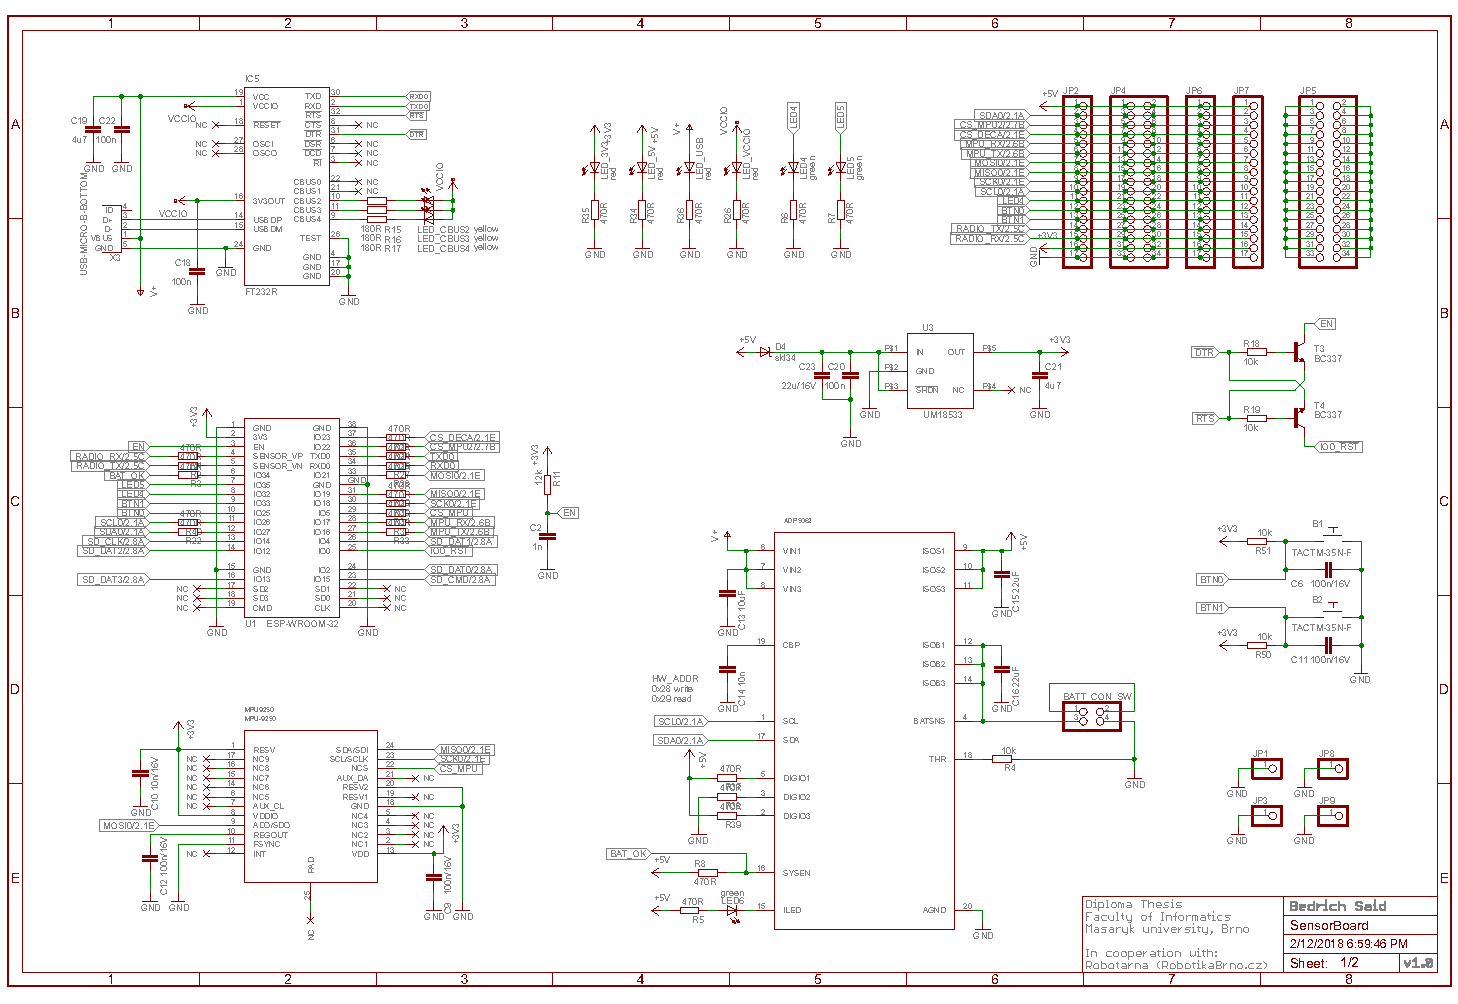
\includegraphics[angle=90, scale=1]{img/sch1.pdf}
	\label{sch1}
	\caption{Schematics of the Sensor Board sheet 1}
\end{figure}

\begin{figure}
	\centering
	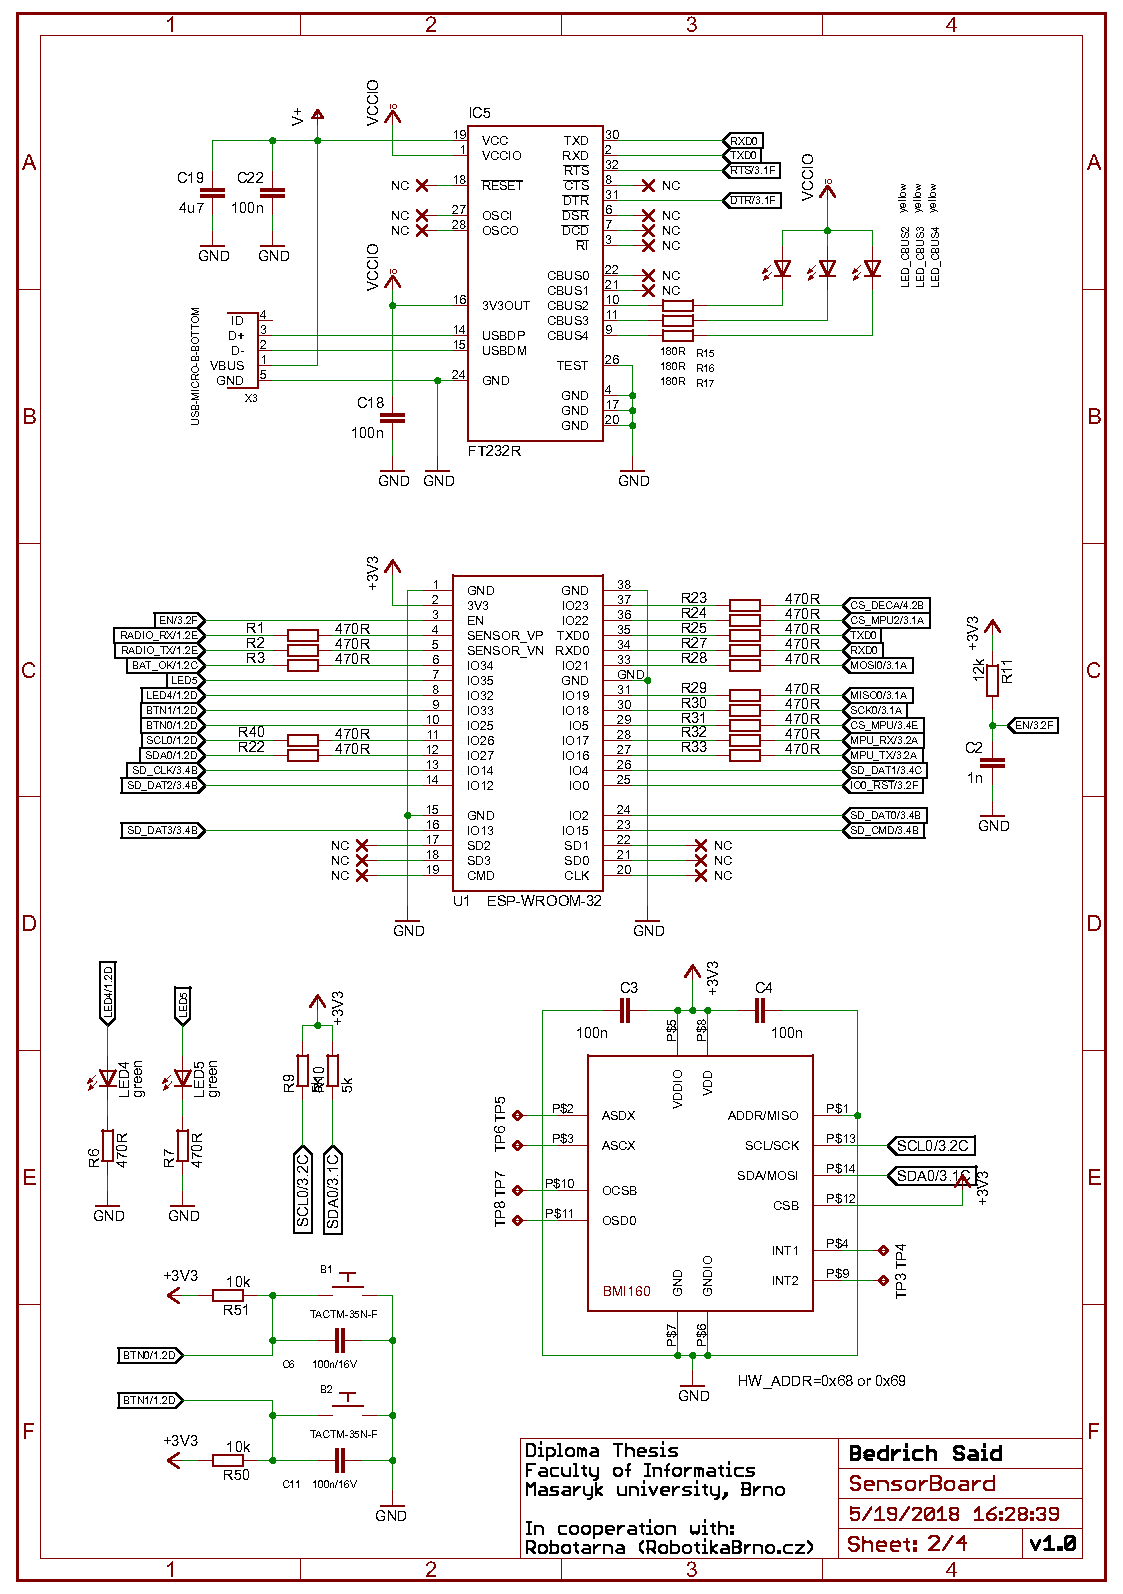
\includegraphics[angle=90, scale=1]{img/sch2.pdf}
	\label{sch2}
	\caption{Schematics of the Sensor Board sheet 2}
\end{figure}

\subsection{Board layout}
//todo: text

\begin{figure}
	\centering
	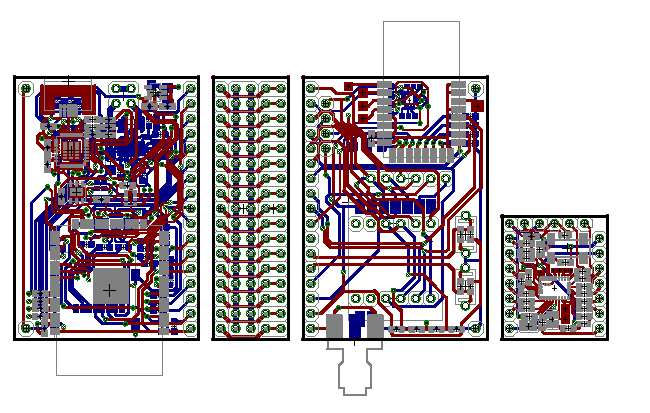
\includegraphics[scale=1]{img/brd.pdf}
	\begin{center}
		Top and Bottom layer
	\end{center}
	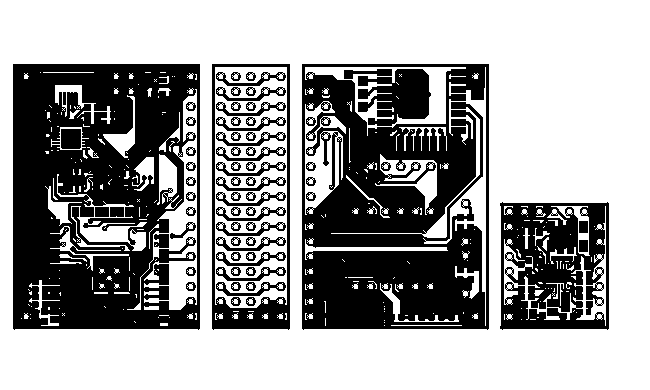
\includegraphics[scale=1]{img/brdTop.pdf}
	\begin{center}
		Only Top layer
	\end{center}
	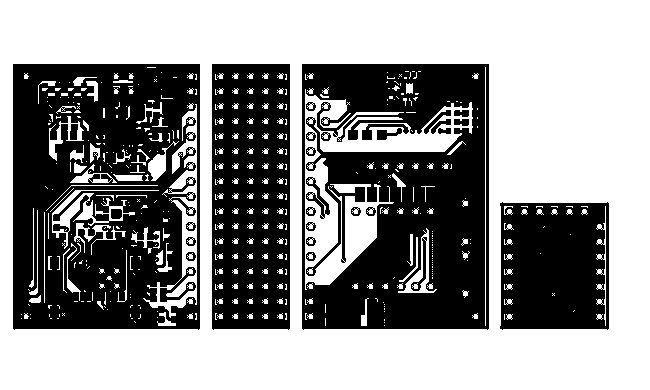
\includegraphics[scale=1]{img/brdBottom.pdf}
	\begin{center}
		Only Bottom layer
	\end{center}
	\label{brd1}
	\caption{Sensor Board layout in scale 1:1}
\end{figure}

\begin{figure}
	\centering
	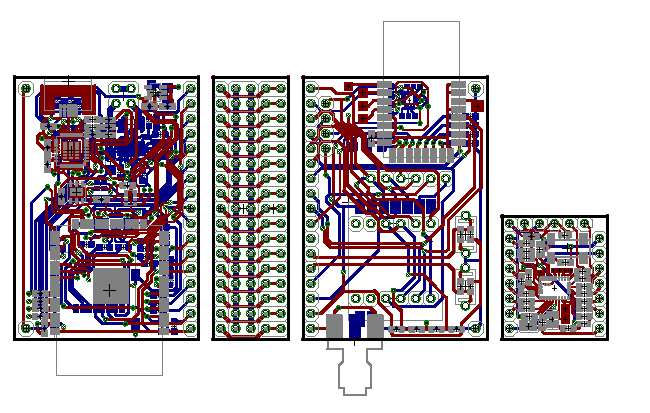
\includegraphics[angle=90, scale=2]{img/brd.pdf}
	\label{brd2}
	\caption{Sensor Board layout in detail scale 2:1}
\end{figure}

\subsection{Mechanical layout and connectors}
//todo: obrazek SVG

\section{Manufacturing}
//todo: text: postup výroby



\section{Testing}

\subsection{Errata}
The table //todo shows all errors I have found in the Sensor Board prototype.

//todo: tabulka errata
- můstek pod USB konektorem
- prohozené MOSI MISO oproti standardu
- jedna LED na pouze input pinu, takže nefunkční
- pull-up resistory na SD kartě
- teploměr příliš blízko procesoru, je ovlivňován teplem generovaným procesorem

\section{Recommendations for the next version}

//todo: itemize
- signalizační RGB LED místo několika klasických, klidně víc inteligentních LED
- přesunout všechny IMU výpočty do BMF055 a ESP32 nechat pouze pro komunikaci a uživatelský kód, klidně připojit senzory k BMF055 místo přímo k ESP32
- design jako vícevrstvou desku s hustším pokrytím součástek, případně součástky na jedné straně a na druhé baterii
- oddělit na desce prostor pro senzory a prostor pro součástky, které generují víc tepla
- totéž pro napájení, zvlášť napájení pro senzory a pro komunikaci/výpočty
- zvážit širší možnosti USB konektoru, třeba USB host nebo USB-C, případně kombinovaná sériová linka a přenos souborů z SD karty
- testpady pro osciloskop

\end{document}